\documentclass{report}

\usepackage{array}
\usepackage{booktabs}  % For better table formatting
\usepackage{amsmath}
\usepackage{geometry}
\usepackage{graphicx}

% Define a custom environment with reduced margins
\usepackage{changepage}

\newenvironment{narrowmargins}{
    \begin{adjustwidth}{-0.75in}{0.25in} % Adjust the left and right margins by 0.5in
}{
    \end{adjustwidth}
}
\counterwithin{figure}{subsection}

\title{Implementation Report Analysis}
\author{Vivado}
\date{\today}

\begin{document}
\maketitle

\chapter{Introduction}

This document is an analysis of the implementation report generated by Vivado for the \texttt{top} module. The report is generated after the implementation process is completed. The report contains information about the resources used by the design, the timing constraints, and the timing performance of the design. The report is used to analyze the design and to identify any potential issues that may need to be addressed.

\chapter{Resource Utilization}

The resource utilization section of the report provides information about the resources used by the design. This includes information about the number of LUTs, FFs, BRAMs, and DSPs used by the design. The resource utilization section also provides information about the number of IOBs used by the design.

\section{Common Resource Types}
Here are some common resource types used in FPGA designs and Verilog codes that utilizes these resources:
\subsection{LUTs}
LUTs (Look-Up Tables) are fundamental building blocks in FPGA designs. They are used to implement combinational logic functions. Each LUT has a fixed number of inputs and a single output. The Verilog code snippet below shows an example of a 2-input LUT implementation:

\begin{verbatim}
module lut2 (input wire a, b, output wire y);
    assign y = a & b;
endmodule
\end{verbatim}

\begin{figure}[ht]
    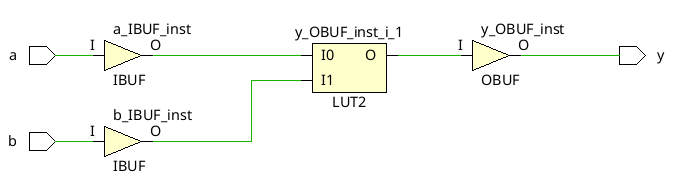
\includegraphics[width=0.6\linewidth]{images/lut.png}
    \centering
    \caption{LUT Implemented}
    \label{fig:lut}
\end{figure}

\subsection{FFs}
FFs (Flip-Flops) are sequential elements used to store and propagate data in FPGA designs. They are commonly used to implement registers and memory elements. The Verilog code snippet below shows an example of a D flip-flop implementation:

\begin{verbatim}
module dff (input wire clk, reset, input wire d, output reg q);
    always @(posedge clk or posedge reset)
        if (reset)
            q <= 1'b0;
        else
            q <= d;
endmodule
\end{verbatim}

\begin{figure}[ht]
    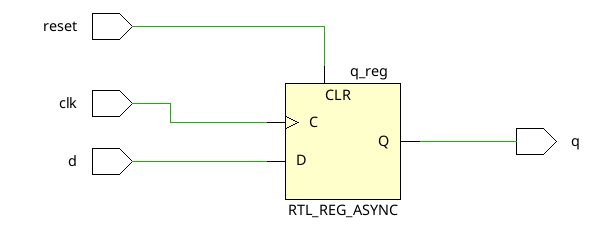
\includegraphics[width=0.6\linewidth]{images/ff.png}
    \centering
    \caption{FF Synthesised}
    \label{fig:ff}
\end{figure}

\subsection{BRAMs}
BRAMs (Block RAMs) are memory elements in FPGA designs. They provide large storage capacity and high-speed access. They can be coded into fpga, or The Verilog code snippet below shows an example of a simple dual-port RAM implementation:
\begin{verbatim}
module dual_port_ram (
    input wire clk,
    input wire [7:0] addr_a, addr_b,
    input wire [7:0] data_a, data_b,
    input wire we_a, we_b,
    output reg [7:0] q_a, q_b
);
    reg [7:0] mem [0:255];
    always @(posedge clk) begin
        if (we_a)
            mem[addr_a] <= data_a;
        q_a <= mem[addr_a]; // Synchronous read for port A
    end
    always @(posedge clk) begin
        if (we_b)
            mem[addr_b] <= data_b;
        q_b <= mem[addr_b]; // Synchronous read for port B
    end
endmodule
\end{verbatim}

* Vivado can pick BRAM, LUTRAM, or FFs to implement your design. If you want to force Vivado to use BRAM, you can use \texttt{(* ram\_style = "block" *)} in the module. If your design fits Bram conditions, Vivado will use BRAMs to implement your design. If you do not explicitly specify, Vivado will use LUTRAMs or FFs to implement your design depending on size required access speed etc.

\begin{figure}[ht]
    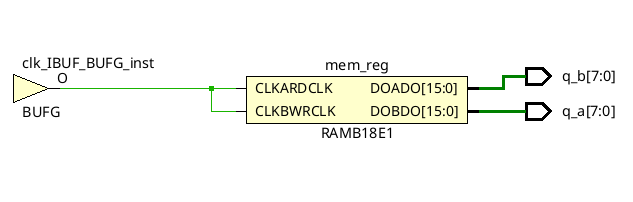
\includegraphics[width=0.6\linewidth]{images/bram.png}
    \centering
    \caption{BRam Implemented}
    \label{fig:bram}
\end{figure}

\subsection{DSPs}
DSPs (Digital Signal Processors) are specialized hardware blocks in FPGA designs used for high-performance signal processing operations. They are commonly used in applications such as image and audio processing. The Verilog code snippet below shows an example of a simple multiplier using DSP blocks:

\begin{verbatim}
module multiplier (input wire [9:0] a, b, output wire [19:0] result);
    assign result = a * b;
endmodule
\end{verbatim}
\begin{figure}[ht]
    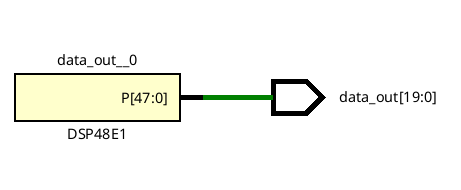
\includegraphics[width=0.6\linewidth]{images/dsp.png}
    \centering
    \caption{DSP Block Implemented}
    \label{fig:dsp}
\end{figure}

*For Basys3 Vivado prefers to use dsp blocks 10 and more bits multiplication. For 9 bits and less, it uses LUTs and FFs, but adding \texttt{(* use\_dsp = "yes" *)} to the module can force Vivado to DSP for arithmetic operations.

\subsection{IOBs}
IOBs (Input/Output Blocks) are used to interface the FPGA design with external devices. They provide the necessary logic to drive and receive signals from the external world. The Verilog code snippet below shows an example of an IOB implementation for a simple GPIO (General Purpose Input/Output) interface:

\begin{verbatim}
module gpio (input wire clk, input wire reset, input wire [7:0] data_in,
             output wire [7:0] data_out, inout wire [7:0] io_pins);
    reg [7:0] internal_reg;
    
    always @(posedge clk or posedge reset)
        if (reset)
            internal_reg <= 8'b0;
        else
            internal_reg <= data_in;
    
    assign data_out = internal_reg;
    assign io_pins = internal_reg;
endmodule
\end{verbatim}

\section{Resource Utilization Report}

The resource utilization report provides information about how many of these components are available in the FPGA and how many are used by your design. It helps you understand how efficiently your design is utilizing the available resources and whether any adjustments or optimizations are needed.

\paragraph{There are 8 parts in the resource utilization report.}
\begin{enumerate}
    \item Slice Logic: How many LUTs and FFs are used in the design. How many of LUTs are used as Logic or Memory and how many of FFs are used as Registers or Latches.
    \item Slice Logic Distribution: How the LUTs and FFs are distributed across the slices.
    \item Memory: Usage report of build in memory blocks. There can be different types for different fpga families.
    \item DSPs: Usage report of DSP blocks.
    \item IOs
    \item BUFG/BUFGCTRL (Clocking): Usage report of clocking resources.
    \item Specific Feature: Usage report of specific featured blocks of the fpga card.
    \item Primitive: How many of each primitive type are utilized in your design. A more detailed report of the sources mentioned in the other tables used in the design. It doesn't give the utilization ratio.
\end{enumerate}

Example scenarios to chose which part to look at:
\begin{itemize}
    \item If you wanted to know exactly how many flip-flops or LUTs of a particular configuration (like FDRE for a flip-flop with enable) were used, you would consult the Primitive Types Report.
    \item If the design is using a lot of memory resources as LUT, you may want to look at the Memory section to see if there are any optimizations that can be made.
    \item If the design is using a lot math operations, you may want to look at the DSP and LUT section to see if the design is close to the limits.
    \item \textbf{***The synthesis tool might not be able to utilize the desing as desired. A different block of fpga can be used to implement your design. For example a buffer can be utilized in BRAMs, LUTRAMs, or FFs. Simple changes in your design can make implementation tool to chose a different resource. ***} 
\end{itemize}
An example table from resource utilization report for the \texttt{top} module is shown below:


\begin{verbatim}
    8. Primitives
    -------------
    
    +----------+------+---------------------+
    | Ref Name | Used | Functional Category |
    +----------+------+---------------------+
    | FDRE     |  178 |        Flop & Latch |
    | LUT6     |   79 |                 LUT |
    | LUT4     |   48 |                 LUT |
    | LUT5     |   22 |                 LUT |
    | LUT2     |   21 |                 LUT |
    | LUT3     |   18 |                 LUT |
    | CARRY4   |   11 |          CarryLogic |
    | FDSE     |   10 |        Flop & Latch |
    | OBUF     |    7 |                  IO |
    | RAMB18E1 |    4 |        Block Memory |
    | IBUF     |    3 |                  IO |
    | LUT1     |    2 |                 LUT |
    | BUFG     |    2 |               Clock |
    +----------+------+---------------------+
    
\end{verbatim}

General file names for this report are \texttt{Module\_Name\_utilization\_routed.rpt} or \texttt{Module\_Name\_utilization\_placed.rpt}.

\subsection{TCL Commands}
The most useful setting for utilization analysis when calling tcl option is hierarchical. This option gives a single table report, but with primitive types used by all submodules and theirs. This is useful to see which module is using the most of a specific resource. You can set this setting in the tcl command as follows:

\begin{verbatim}
    report_utilization -hierarchical
\end{verbatim}

*This command can help you to see which module is using the most of a specific resource. If you see a module is using a lot of a specific resource, you can optimize that module to reduce the resource usage.

\chapter{Power Analysis}
Power analysis is an important aspect of FPGA design as it helps in understanding the power consumption of the implemented design. By analyzing the power utilization, we can optimize the design to reduce power consumption and improve overall efficiency. Power analysis provides insights into the power consumption of different components in the design, such as LUTs, FFs, BRAMs, DSPs, and IOBs. It also helps in identifying any potential power-related issues that may need to be addressed. In this section, we will explore the power utilization of the \texttt{top} module and analyze the power consumption of various components in the design.

\section{Power Utilization Report}
The power utilization report provides information about the power consumption of different components in the design. It includes details about the dynamic power, static power, and total power consumption of the design. 
There are 3 parts in the power utilization report. The content of the report may vary depending on the FPGA family and the tool used. \paragraph{However, The first two table \(1.1\ and\  1.2\) and the last table \(3.1\) are the most useful table for power analysis.} 
\begin{itemize}
    \item 1.1 Power Summary: This table provides an overview of the power consumption of the design. It includes information about the dynamic power, static power, dynamic power, and total power consumption of the design. It also provides details about constraints (if you set).
    \item 1.2 Power by Component: This table provides detailed information about the power consumption of different components in the design. It includes information about the power consumption of LUTs, FFs, BRAMs, DSPs, and IOBs. It helps in understanding the power consumption of different components and optimizing the design to reduce power consumption.
    \item 3.1 Power by Hierarchy: This table provides a hierarchical view of the power consumption of the design. It includes information about the power consumption of different modules in the design and helps in identifying the power consumption of individual modules.
\end{itemize}

\subsection{Power Summary (1.1)}
An example table from power utilization report for the \texttt{top} module is shown below:

\begin{verbatim}
    +--------------------------+--------------+
| Total On-Chip Power (W)  | 0.082        |
| Design Power Budget (W)  | Unspecified* |
| Power Budget Margin (W)  | NA           |
| Dynamic (W)              | 0.010        |
| Device Static (W)        | 0.072        |
| Effective TJA (C/W)      | 5.0          |
| Max Ambient (C)          | 84.6         |
| Junction Temperature (C) | 25.4         |
| Confidence Level         | Medium       |
| Setting File             | ---          |
| Simulation Activity File | ---          |
| Design Nets Matched      | NA           |
+--------------------------+--------------+
\end{verbatim}

An explanation of the fields and tips about some fields in the table is as follows:
\begin{itemize}
    \item Total On-Chip Power (W): The total power consumption of the design on the FPGA chip.
    \item Design Power Budget (W): The specified power budget for the design. \textbf{If you set a power budget, you can compare the actual power consumption with the specified power budget to ensure that the design meets the power requirements. If you need to run on battery power, this might be important.}
    \item Power Budget Margin (W): The margin between the actual power consumption and the specified power budget.
    \item Dynamic (W): The dynamic power consumption of the design. \textbf{High dynamic power drawn when performance required. It is best to keep power drawn low when not required. For example, if your design uses multiple modules used as needed, you can disable their clocks when they are not used. This should reduce dynamic power.}
    \item Device Static (W): The static power consumption of the FPGA device. \textbf{This should be reduced to keep power consumption and temperature low. Power gating can be used to reduce static power. This is not available for all FPGAs please research.}
    \item Effective TJA (C/W): The thermal junction-to-ambient resistance of the FPGA device.
    \item Max Ambient (C): The maximum ambient temperature for the design.
    \item Junction Temperature (C): The junction temperature of the FPGA device.
    \item Confidence Level: The confidence level of the power analysis results. This depends on the user specifications. \textbf{If you want a more accurate result, you can increase the confidence level by setting io and clock activity using GUI or constraints file.}
    \item Setting File: The settings file used for the power analysis.
    \item Simulation Activity File: The simulation activity file used for the power analysis.
    \item Design Nets Matched: The number of design nets matched during the power analysis.
\end{itemize}

\subsection{Power by Component (1.2)}
An example table from power utilization report for the \texttt{top} module is shown below:
\begin{verbatim}
+----------------+-----------+----------+-----------+-----------------+
| On-Chip        | Power (W) | Used     | Available | Utilization (%) |
+----------------+-----------+----------+-----------+-----------------+
| Clocks         |     0.001 |        5 |       --- |             --- |
| Slice Logic    |    <0.001 |      406 |       --- |             --- |
|   LUT as Logic |    <0.001 |      164 |     20800 |            0.79 |
|   Register     |    <0.001 |      188 |     41600 |            0.45 |
|   CARRY4       |    <0.001 |       11 |      8150 |            0.13 |
|   Others       |     0.000 |       17 |       --- |             --- |
| Signals        |    <0.001 |      363 |       --- |             --- |
| Block RAM      |    <0.001 |        2 |        50 |            4.00 |
| I/O            |     0.007 |       10 |       106 |            9.43 |
| Static Power   |     0.072 |          |           |                 |
| Total          |     0.082 |          |           |                 |
+----------------+-----------+----------+-----------+-----------------+
\end{verbatim}
Using this table and information from the previous section, you can analyze the power consumption of different components in the design and identify areas where power optimization is needed. For example, if the design is using a large number of LUTs, you can optimize the design to reduce the number of LUTs used and reduce power consumption. Similarly, if the design is using a large number of a component, and if it is more efficient to use other blocks you can force to use other blocks for your design.

\subsection{Power by Hierarchy (3.1)}
An example table from power utilization report for the \texttt{top} module is shown below:
\begin{verbatim}
+---------------+-----------+
| Name          | Power (W) |
+---------------+-----------+
| MemController |     0.010 |
+---------------+-----------+
\end{verbatim}
This table is not a great example,but if yours include your sub modules you can analyze the power consumption of different modules in the design and identify areas where power optimization is needed. For example, if a particular module is consuming a large amount of power, you can optimize that module to reduce power consumption. This because of the hierarchical depth setting. At next session you will see how to set this setting.
\subsection{TCL Commands}
The most useful setting for power analysis when calling tcl option is hierarchical\_depth. When implem run it ussually set to 1 by default. However, if you set it to 0, you can see the power consumption of the submodules and their submodules until the least piece. This is useful to see which module is consuming the most power, or you can set the depth you desire You can set this setting in the tcl command as follows:

\begin{verbatim}
    report_power -hierarchical_depth 0
\end{verbatim}

\chapter{Methodology Warnings}
The methodology warnings section of the report provides information about any potential issues or warnings that may need to be addressed. This section includes information about the timing constraints, clock constraints, and other design constraints that may impact the performance of the design. The methodology warnings section helps in identifying any potential issues that may need to be addressed to improve the performance of the design.

\section{Methodology Warnings Report}
Example issues from methodology warnings report for the \texttt{top} module is shown below:
\begin{verbatim}
    [Timing 38-282] The design failed to meet the timing requirements. 
    Please see the timing summary report for details on the timing violations.

    [Place 30-58] IO placement is not user specified.

    TIMING-18#1 Warning
    Missing input or output delay  
    An input delay is missing on reset relative to the rising and/or falling clock edge(s) 
    of sys_clk_pin.
    Related violations: <none>
\end{verbatim}
Some of this issues are about the constraints that you did not set. Some can be ignored if you are confident about timing latency of those pins. However, if you are not sure about the latency of the pins, you can set the constraints for those pins. Then if you get timing failed warning, your system will be high probably not working as desired stably. IO placement is more important, there might be bitstream write issues even if it is implemented. Also, if the tool can place as it wants, the design may not function as desired on the device. You can check the io placement in \texttt{Module\_Name\_io\_placed.rpt} file.

\chapter{Timing Analysis}
The timing analysis section of the report provides information about the timing performance of the design. This includes information about the clock constraints, setup and hold times, clock-to-q delays, and other timing parameters that impact the performance of the design. The timing analysis section helps in identifying any potential timing issues that may need to be addressed to improve the performance of the design. This is the most complex and important part of the report.
\section{Definitions and Explanations}
These are some common terms used in the timing analysis report in order to understand the report better:
\begin{itemize}
    \item \textbf{Setup Time:} The amount of time the input signal must be stable before the active edge of the clock signal. If the input signal changes too close to the active edge of the clock signal, the flip-flop may not capture the correct value.
    \item \textbf{Hold Time:} The amount of time the input signal must be stable after the active edge of the clock signal. If the input signal changes too soon after the active edge of the clock signal, the flip-flop may not capture the correct value.
    \item \textbf{Slack:} The slack is the amount of time by which the actual timing of the design exceeds the required timing. A positive slack indicates that the design meets the timing requirements, while a negative slack indicates that the design fails to meet the timing requirements.
    \item \textbf{Clock-to-Q Delay:} The amount of time it takes for the output signal to change after the active edge of the clock signal. This is the delay through the flip-flop.
    \item \textbf{Clock Skew:} The difference in arrival times of the clock signal at different flip-flops. Clock skew can cause timing violations if the clock signal arrives at different flip-flops at different times.
    \item \textbf{Clock Uncertainty:} The amount of uncertainty in the clock signal arrival time. Clock uncertainty can cause timing violations if the clock signal arrives at different flip-flops at different times.
    \item \textbf{Critical Path:} The path in the design with the longest delay. The critical path determines the maximum clock frequency of the design.
    \item \textbf{Timing Violation:} A timing violation occurs when the design fails to meet the timing requirements specified in the constraints file. Timing violations can cause the design to malfunction or fail to meet the desired performance.
    \item \textbf{Clock Domain Crossing:} Clock domain crossing occurs when signals from one clock domain are transferred to another clock domain. Clock domain crossing can cause timing violations if the signals are not synchronized properly.
    \item \textbf{False Path:} A false path is a path in the design that is not required to meet the timing requirements. False paths are ignored by the timing analysis tool to reduce the analysis time.
    \item \textbf{TNS: } Total Negative Slack. The sum of all negative slack values in the design.
    \item \textbf{WNS: } Worst Negative Slack. The worst negative slack value in the design.
    \item \textbf{THS: } Total Hold Slack. The sum of all hold slack values in the design.
    \item \textbf{WHS: } Worst Hold Slack. The worst hold slack value in the design.
    \item \textbf{WPWS: } Worst Pulse Width Slack. The worst pulse width slack value in the design.
    \item \textbf{Data Path Delay: } The amount of time it takes for the data signal to propagate through the combinational logic in the design. Data path delay is a critical parameter that impacts the overall performance of the design.
    \item \textbf{System Jitter: } The amount of variation in the clock signal arrival time. System jitter can cause timing violations if the clock signal arrives at different flip-flops at different times.
    \item \textbf{Input Jitter: } The amount of variation in the input signal arrival time. Input jitter can cause timing violations if the input signal changes too close to the active edge of the clock signal.
\end{itemize}
\section{Calculation of Slack}
The slack is calculated as follows:
\begin{verbatim}
    Time Avaliable for Data Setup = Clock Period - Data Path Delay
    Setup Slack = (Clock Period) - (Time Avaliable for Data Setup)

    Time Avaliable for Data Hold = Data Change Time after Clock Edge
    Hold Slack = Time Avaliable for Data Hold - Hold Time

    Time Required = Time Required for Pulse to be High 
    Actual Pulse Width = Time that the Pulse is High
    Pulse Width Slack = Actual Pulse Width - Time Required
\end{verbatim}
\section{Timing Analysis Report}
The timing analysis doesn't have expilicit sections like the other reports. It is a long report that includes all the timing information of the design. However, we can break it down into 4 parts:

\subsection{Timing Checks}
At the start of the timing analysis report, there is a summary of the timing checks. These checks make sure that an accurate timing report is produced. The summary provides timing warnings for your design. This suggestions might be useful to fix the timing issues.
An example from the timing analysis report for the \texttt{top} module is shown below:
\begin{verbatim}
    Table of Contents
    -----------------
    1. checking no_clock (0)
    2. checking constant_clock (0)
    3. checking pulse_width_clock (0)
    4. checking unconstrained_internal_endpoints (0)
    5. checking no_input_delay (2)
    6. checking no_output_delay (6)
    7. checking multiple_clock (0)
    8. checking generated_clocks (0)
    9. checking loops (0)
    10. checking partial_input_delay (0)
    11. checking partial_output_delay (0)
    12. checking latch_loops (0)
    
    1. checking no_clock (0)
    ------------------------
     There are 0 register/latch pins with no clock.
    
    
    2. checking constant_clock (0)
    ------------------------------
     There are 0 register/latch pins with constant_clock.
    
    
    3. checking pulse_width_clock (0)
    ---------------------------------
     There are 0 register/latch pins which need pulse_width check
    
    
    4. checking unconstrained_internal_endpoints (0)
    ------------------------------------------------
     There are 0 pins that are not constrained for maximum delay.
    
     There are 0 pins that are not constrained for maximum delay due to constant clock.
    
    
    5. checking no_input_delay (2)
    ------------------------------
     There are 2 input ports with no input delay specified. (HIGH)
    
     There are 0 input ports with no input delay but user has a false path constraint.
    
    
    6. checking no_output_delay (6)
    -------------------------------
     There are 6 ports with no output delay specified. (HIGH)
    
     There are 0 ports with no output delay but user has a false path constraint
    
     There are 0 ports with no output delay but with a timing clock defined on it 
     or propagating through it
    
    
    7. checking multiple_clock (0)
    ------------------------------
     There are 0 register/latch pins with multiple clocks.
    
    
    8. checking generated_clocks (0)
    --------------------------------
     There are 0 generated clocks that are not connected to a clock source.
    
    
    9. checking loops (0)
    ---------------------
     There are 0 combinational loops in the design.
    
    
    10. checking partial_input_delay (0)
    ------------------------------------
     There are 0 input ports with partial input delay specified.
    
    
    11. checking partial_output_delay (0)
    -------------------------------------
     There are 0 ports with partial output delay specified.
    
    
    12. checking latch_loops (0)
    ----------------------------
     There are 0 combinational latch loops in the design through latch input
\end{verbatim}
Using this information, you can identify any potential timing issues in the design and take appropriate actions to address them. For example, if there are input ports with no input delay specified, you can set the input delay constraints to ensure that the design meets the timing requirements.
If the design has a negative slack, the input delay that is not specified might be causing this result.
This warnings effect the detailed design timing summary which comes after.

\subsection{Design Timing Summary}
After the checks, there is a timing report of the whole module.
An example from the timing analysis report for this part is shown below:

\begin{verbatim}
----------------------------------------------------------------------------------
| Design Timing Summary                                                          |
| ---------------------                                                          |
----------------------------------------------------------------------------------

WNS(ns)      TNS(ns)  TNS Failing Endpoints  TNS Total Endpoints      WHS(ns)      
-------      -------  ---------------------  -------------------      -------
3.864        0.000                      0                  561        0.058

THS(ns)  THS Failing Endpoints  THS Total Endpoints     WPWS(ns)     TPWS(ns)  
-------  ---------------------  -------------------     --------     -------- 
0.000                      0                  561        4.500        0.000   

TPWS Failing Endpoints  TPWS Total Endpoints  
----------------------  --------------------
                     0                   198    
\end{verbatim}

The titles are already explained in the previous part. If there is no negative value or close to zero, the design is working as desired. If there is a negative value, you should check the detailed timing report to see which part of the design is causing the issue.
Hold times are close to zero, but they are how they are suppose to be as hold time is already a small value.

\subsection{Clock Timing Summary}
After the design timing summary, there is a clock timing summary. This part provides information about the clock constraints, slacks for each clock's own domain, slacks between clock domains, and clock uncertainty of the design. It helps in understanding the clock performance of the design and identifying any potential clock-related issues that may need to be addressed.
An example from the timing analysis report for this part is shown below:

\begin{verbatim}
------------------------------------------------------------------------------------------------
| Clock Summary
| -------------
------------------------------------------------------------------------------------------------

Clock        Waveform(ns)           Period(ns)      Frequency(MHz)
-----        ------------           ----------      --------------
sys_clk_pin  {0.000 5.000}          10.000          100.000         
    rx_clk     {0.000 270.000}        540.000         1.852           
    tx_clk     {0.000 4340.000}       8680.000        0.115           

    
------------------------------------------------------------------------------------------------
| Intra Clock Table
| -----------------
------------------------------------------------------------------------------------------------

Clock             WNS(ns)      TNS(ns)  TNS Failing Endpoints  TNS Total Endpoints
-----             -------      -------  ---------------------  -------------------
sys_clk_pin         4.227        0.000                      0                  445
rx_clk            535.110        0.000                      0                   74
tx_clk           8675.541        0.000                      0                   34

WHS(ns)      THS(ns)  THS Failing Endpoints  THS Total Endpoints     WPWS(ns)
-------      -------  ---------------------  -------------------     --------
0.058        0.000                      0                  445        4.500
0.177        0.000                      0                   74      269.500
0.191        0.000                      0                   34     4339.500

TPWS(ns)  TPWS Failing Endpoints  TPWS Total Endpoints  
--------  ----------------------  --------------------  
0.000                       0                   140  
0.000                       0                    40
0.000                       0                    18      
-------------------------------------------------------------
| Inter Clock Table                                         |
| -----------------                                         |
-------------------------------------------------------------

From Clock    To Clock          WNS(ns)      TNS(ns)  TNS Failing Endpoints
----------    --------          -------      -------  ---------------------
rx_clk        sys_clk_pin         3.864        0.000                      0
tx_clk        sys_clk_pin         5.181        0.000                      0
sys_clk_pin   tx_clk              6.771        0.000                      0

TNS Total Endpoints      WHS(ns)      THS(ns)  THS Failing Endpoints
-------------------      -------      -------  ---------------------
                69        0.945        0.000                      0             
                 5        0.747        0.000                      0                    
                25        0.131        0.000                      0                       

                    THS Total Endpoints
                    -------------------    
                                    69
                                     5
                                    25
    
\end{verbatim}
The first table in this part gives wave specifications of the clocks. The second table gives the slack values of the clocks. The third table gives the slack values between the clocks. If there is a negative value in the slack, you should check the detailed timing report to see which part of the design is causing the issue.

As you can realize slower clocks has no problem with timing as they have a lot of slack. However, the faster clock has a tight timing. This is a common issue in the designs.

Inter Clock table is formed by the clocks that are crossing each other. If two systems with different clocks are not connected at all, they are not in this table. If they are connected in a way (output/input), it is in this table.
From this report, we can understand that the module with main clock both reads and writes to the module with tx\_clk in always @(clk) block.                                                                                                                                                                                                                                                        

When a design slack problem is detected, the first thing to do is to check the detailed timing report to see which part or module interaction of the design is causing the issue.

\subsection{Detailed Timing Report}
For each clock domain and cross domain, for each path the timing report is placed here ordered slack worst to best. All component's delay on the path can be seen with input and clock jitter calculation available.
An example part from the timing analysis report for this part    is shown below (For single path):

\begin{narrowmargins}
\begin{verbatim}
Slack (MET) :             4.227ns  (required time - arrival time)
Source:                 time_out_counter_reg[12]/C
                        (rising edge-triggered cell FDRE clocked by sys_clk_pin  {rise@0.000ns fall@5.000ns period=10.000ns})
Destination:            time_out_counter_reg[24]/R
                        (rising edge-triggered cell FDRE clocked by sys_clk_pin  {rise@0.000ns fall@5.000ns period=10.000ns})
Path Group:             sys_clk_pin
Path Type:              Setup (Max at Slow Process Corner)
Requirement:            10.000ns  (sys_clk_pin rise@10.000ns - sys_clk_pin rise@0.000ns)
Data Path Delay:        5.188ns  (logic 1.014ns (19.546%)  route 4.174ns (80.453%))
Logic Levels:           4  (LUT2=1 LUT3=1 LUT4=1 LUT6=1)
Clock Path Skew:        -0.026ns (DCD - SCD + CPR)
Destination Clock Delay (DCD):    4.857ns = ( 14.857 - 10.000 ) 
Source Clock Delay      (SCD):    5.156ns
Clock Pessimism Removal (CPR):    0.273ns
Clock Uncertainty:      0.035ns  ((TSJ^2 + TIJ^2)^1/2 + DJ) / 2 + PE
Total System Jitter     (TSJ):    0.071ns
Total Input Jitter      (TIJ):    0.000ns
Discrete Jitter          (DJ):    0.000ns
Phase Error              (PE):    0.000ns

Location             Delay type                Incr(ns)  Path(ns)    Netlist Resource(s)
-------------------------------------------------------------------    -------------------
                        (clock sys_clk_pin rise edge)
                                                    0.000     0.000 r  
W5                                                0.000     0.000 r  clk (IN)
                        net (fo=0)                   0.000     0.000    clk
W5                   IBUF (Prop_ibuf_I_O)         1.458     1.458 r  clk_IBUF_inst/O
                        net (fo=1, routed)           1.967     3.425    clk_IBUF
BUFGCTRL_X0Y0        BUFG (Prop_bufg_I_O)         0.096     3.521 r  clk_IBUF_BUFG_inst/O
                        net (fo=139, routed)         1.635     5.156    clk_IBUF_BUFG
SLICE_X6Y4           FDRE                                         r  time_out_counter_reg[12]/C
-------------------------------------------------------------------    -------------------
SLICE_X6Y4           FDRE (Prop_fdre_C_Q)         0.518     5.674 f  time_out_counter_reg[12]/Q
                        net (fo=2, routed)           0.653     6.328    nolabel_line102/time_out_counter[0]_i_2_5[3]
SLICE_X7Y5           LUT4 (Prop_lut4_I0_O)        0.124     6.452 f  nolabel_line102/time_out_counter[0]_i_6/O
                        net (fo=1, routed)           1.154     7.605    nolabel_line102/time_out_counter[0]_i_6_n_0
SLICE_X7Y5           LUT6 (Prop_lut6_I3_O)        0.124     7.729 f  nolabel_line102/time_out_counter[0]_i_2/O
                        net (fo=3, routed)           0.597     8.327    nolabel_line102/time_out_counter[0]_i_2_n_0
SLICE_X9Y5           LUT2 (Prop_lut2_I0_O)        0.124     8.451 f  nolabel_line102/FSM_sequential_state[2]_i_2/O
                        net (fo=4, routed)           0.898     9.349    nolabel_line102/time_out_counter_reg[0]
SLICE_X7Y4           LUT3 (Prop_lut3_I2_O)        0.124     9.473 r  nolabel_line102/time_out_counter[26]_i_1/O
                        net (fo=26, routed)          0.871    10.344    nolabel_line102_n_21
SLICE_X6Y7           FDRE                                         r  time_out_counter_reg[24]/R
-------------------------------------------------------------------    -------------------

                        (clock sys_clk_pin rise edge)
                                                    10.000    10.000 r  
W5                                                0.000    10.000 r  clk (IN)
                        net (fo=0)                   0.000    10.000    clk
W5                   IBUF (Prop_ibuf_I_O)         1.388    11.388 r  clk_IBUF_inst/O
                        net (fo=1, routed)           1.862    13.250    clk_IBUF
BUFGCTRL_X0Y0        BUFG (Prop_bufg_I_O)         0.091    13.341 r  clk_IBUF_BUFG_inst/O
                        net (fo=139, routed)         1.516    14.857    clk_IBUF_BUFG
SLICE_X6Y7           FDRE                                         r  time_out_counter_reg[24]/C
                        clock pessimism              0.273    15.130    
                        clock uncertainty           -0.035    15.095    
SLICE_X6Y7           FDRE (Setup_fdre_C_R)       -0.524    14.571    time_out_counter_reg[24]
-------------------------------------------------------------------
                        required time                         14.571    
                        arrival time                         -10.344    
-------------------------------------------------------------------
                        slack                                  4.227  
\end{verbatim}
\end{narrowmargins}
Lets break down the information in the report:

This is a setup timing path. The slack calculated is 4.227ns. This means that the path is 4.227ns faster than the required time. This is a good slack value.
The source and destination of the path are given. The source is the register named \texttt{time\_out\_counter\_reg[12]} that is sending the signal, and the destination is the register named \texttt{time\_out\_counter\_reg[24]} that is receiving the signal.
There are calculation logic between these two registers. Now lets look at times:
\begin{itemize}
    \item Event: Clock Rised at 0.000ns
    \item Clock signal reached the source register at 5.156ns (Source Clock Delay), starting logic flow.
    \item Then the signal of source register is processed by the logic between and reached the destination register at 10.344ns. (Data Path Delay: 10.344ns - 5.156ns = 5.188ns)
    \item The data already ready for destination to setup.
    \item Event: Clock Rised at 10.000ns again
    \item Clock signal reached the destination register at 14.857 (Destination Clock Delay: 14.857ns - 10ns = 4.857ns), starting setup time.
    \item The setup is ready at 14.571ns, with calculation of clock pessimism and uncertainty. (Slack: 14.571ns - 10.344ns = 4.227ns)
\end{itemize}
*Tip: When you see a border line (seperator) after a row in the path timings, a key event happend which are in the graph below. 


\textbf{To sum up, time required is when the second rise of the clock signal is reaches the destination register. Time arrival is the exact time data gets to D pin. Data path delay is Q to D.} The clock reacjed at different times to the two registers. This a clock skew example.


\text{A graphical representation of the path as follows:}
\begin{figure}[h!]
    \centering
    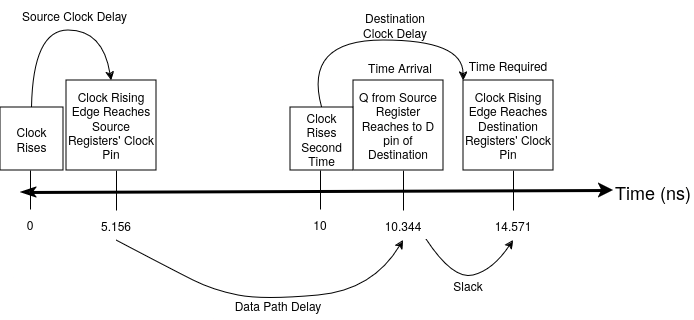
\includegraphics[width=0.9\textwidth]{images/setup_analys.png}
    \caption{Setup Timing Path}
    \label{fig:setup_timing_path}
\end{figure}

When it is a hold slack timing path, the time that data reaches the destination register is calculated. Then the hold time is calculated by the time that data is stable after the clock edge.
Unlike it is given as two flow starting at t = 0ns, one is data path, the other flow includes parts inside the register, which is to find hold time. 
An example hold slack timing path is shown below:

\begin{narrowmargins}
\begin{verbatim}
Min Delay Paths
--------------------------------------------------------------------------------------
Slack (MET) :             0.177ns  (arrival time - required time)
Source:                 nolabel_line85/data_reg_reg[1]/C
                        (rising edge-triggered cell FDSE clocked by rx_clk  {rise@0.000ns fall@270.000ns period=540.000ns})
Destination:            nolabel_line85/data_out_reg[1]/D
                        (rising edge-triggered cell FDRE clocked by rx_clk  {rise@0.000ns fall@270.000ns period=540.000ns})
Path Group:             rx_clk
Path Type:              Hold (Min at Fast Process Corner)
Requirement:            0.000ns  (rx_clk rise@0.000ns - rx_clk rise@0.000ns)
Data Path Delay:        0.266ns  (logic 0.141ns (52.911%)  route 0.125ns (47.089%))
Logic Levels:           0  
Clock Path Skew:        0.013ns (DCD - SCD - CPR)
Destination Clock Delay (DCD):    3.331ns
Source Clock Delay      (SCD):    2.476ns
Clock Pessimism Removal (CPR):    0.842ns

Location             Delay type                Incr(ns)  Path(ns)    Netlist Resource(s)
-------------------------------------------------------------------    -------------------
                     (clock rx_clk rise edge)     0.000     0.000 r  
W5                                                0.000     0.000 r  clk (IN)
                     net (fo=0)                   0.000     0.000    clk
W5                   IBUF (Prop_ibuf_I_O)         0.226     0.226 r  clk_IBUF_inst/O
                     net (fo=1, routed)           0.631     0.858    clk_IBUF
BUFGCTRL_X0Y0        BUFG (Prop_bufg_I_O)         0.026     0.884 r  clk_IBUF_BUFG_inst/O
                     net (fo=139, routed)         0.562     1.445    clk_div/clk_IBUF_BUFG
SLICE_X35Y45         FDRE (Prop_fdre_C_Q)         0.141     1.586 r  clk_div/clk_rx_uart_out_reg/Q
                     net (fo=2, routed)           0.268     1.854    rx_clk
BUFGCTRL_X0Y1        BUFG (Prop_bufg_I_O)         0.026     1.880 r  rx_clk_BUFG_inst/O
                     net (fo=39, routed)          0.596     2.476    nolabel_line85/rx_clk_BUFG
SLICE_X3Y1           FDSE                                         r  nolabel_line85/data_reg_reg[1]/C
-------------------------------------------------------------------    -------------------
SLICE_X3Y1           FDSE (Prop_fdse_C_Q)         0.141     2.617 r  nolabel_line85/data_reg_reg[1]/Q
                     net (fo=2, routed)           0.125     2.742    nolabel_line85/data_reg_reg_n_0_[1]
SLICE_X2Y1           FDRE                                         r  nolabel_line85/data_out_reg[1]/D
-------------------------------------------------------------------    -------------------

                    (clock rx_clk rise edge)     0.000     0.000 r  
W5                                               0.000     0.000 r  clk (IN)
                     net (fo=0)                   0.000     0.000    clk
W5                   IBUF (Prop_ibuf_I_O)         0.414     0.414 r  clk_IBUF_inst/O
                     net (fo=1, routed)           0.685     1.099    clk_IBUF
BUFGCTRL_X0Y0        BUFG (Prop_bufg_I_O)         0.029     1.128 r  clk_IBUF_BUFG_inst/O
                     net (fo=139, routed)         0.831     1.958    clk_div/clk_IBUF_BUFG
SLICE_X35Y45         FDRE (Prop_fdre_C_Q)         0.175     2.133 r  clk_div/clk_rx_uart_out_reg/Q
                     net (fo=2, routed)           0.302     2.436    rx_clk
BUFGCTRL_X0Y1        BUFG (Prop_bufg_I_O)         0.029     2.465 r  rx_clk_BUFG_inst/O
                     net (fo=39, routed)          0.867     3.331    nolabel_line85/rx_clk_BUFG
SLICE_X2Y1           FDRE                                         r  nolabel_line85/data_out_reg[1]/C
                        clock pessimism             -0.842     2.489    
SLICE_X2Y1           FDRE (Hold_fdre_C_D)         0.076     2.565    nolabel_line85/data_out_reg[1]
-------------------------------------------------------------------
                        required time                         -2.565    
                        arrival time                           2.742    
-------------------------------------------------------------------
                        slack                                  0.177    
\end{verbatim}    
\end{narrowmargins}
This report tries to calculate when destination register's data pin is changed after the clock edge for a path.
To break down the information in the report:
\begin{itemize}
    \item Time axis analyzed twice, one for data path, the other for hold time.
    \item The clock signal reached the source register at 2.476ns (Source Clock Delay), starting data path flow.
    \item Then the signal of source register is processed by the logic between and reached the destination register at 2.742ns. (Data Path Delay: 2.742ns - (2.476ns) = 0.266ns)
    \item The data pin is changed 2.742ns after the clock edge.
    \item Time axis analyzed again for hold time. Starting from 0ns, the clock signal reached the destination register at 2.489ns (Destination Clock Delay), starting hold time flow (for previous data that analyzed in setup time, this report looks for future change not back).
    \item After adding the hold time of the destination register, it is found that the data pin must not change before t=2.489ns+0.076ns(Hold Time).
    \item But we already found that the data pin is changed at t=2.742ns. Therefore, the hold slack is calculated as 0.177ns. (Time Arrival - Time Required).
\end{itemize}
\textbf{To sum up, time required is when the destination register completed hold (the data before the current clock rise). Time arrival is the exact time data changes D pin. Data path delay is Q to D.}

\text{A graphical representation of the path as follows:} \pagebreak
\begin{figure}[h!]
    \centering
    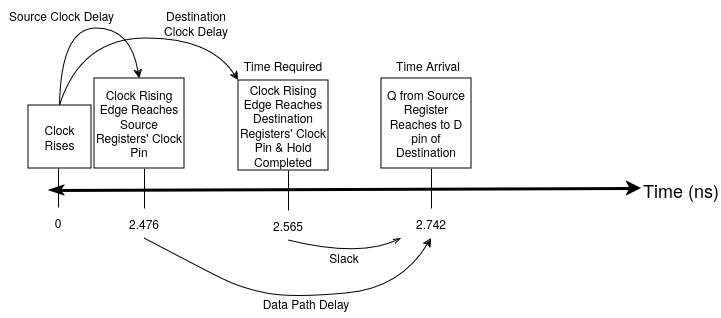
\includegraphics[width=0.9\textwidth]{images/hold_analys.png}
    \caption{Hold Timing Path}
    \label{fig:hold_timing_path}
\end{figure}


As this path reports are categorized by clock, hold and setup, you can find the problematic sequence by inspecting the data path report like above. 
There are several solutions available for negative setup slack:
\begin{itemize}
    \item Add clock buffer to destination clock / Fix clock skew
    \item Optimizing the data path delay
    \item Pipeline the design (insert extra stages/states)
    \item Decrease the clock frequency
\end{itemize}

\textit{*In timing analysis, clock pessimism is initially introduced to ensure safety. However, when calculating timing slack (e.g., setup slack), the tools may apply Clock Pessimism Removal (CPR) to reduce or eliminate some of this conservative estimation. CPR adjusts the clock arrival times so that the analysis is more realistic. Therefore, the slack value is calculated by subtracting the arrival time from the required time. Don't get confused.}

\subsection{Input Delays and Importance to Timing Report}
When input delay is not specified in the constraints file, the tool assumes that the input signal arrives at the flip-flop at the same time as the clock edge, therefore slacks are given infinite. This can cause timing violations if the input signal arrives too close to the clock edge. Therefore, it is important to specify the input delay in the constraints file to ensure that the design meets the timing requirements. This can change:
\begin{itemize}
    \item Your design might have a negative hold slack because of this issue, \textbf{which is not a real issue.}
    \item Your design meet the timing requirements, but \textbf{ with a input delay setup time might be violated in practice.}
\end{itemize}
Therefore, to ensure that design meets the timing requirements in the real world, you should set the input delay in the constraints file.
To set the input delay in the constraints file, you can use the following syntax:
\begin{verbatim}
    set_input_delay -clock [clock_name] -max [delay_value] [port_name]
    set_input_delay -clock [clock_name] -min [delay_value] [port_name]
\end{verbatim}
This is range of delay that input signal can arrive any time inside. For hold time analysis -min is used. For setup time analysis -max is used by Vivado.
\textbf{Testing the effect of input delay to the report}
For this purpose a simple module is created as follows:
\begin{itemize}
    \item Makes calculation using input and writes to a register.
\end{itemize}
\begin{verbatim}
    module InputDelayTest(
        input wire clk,
        input wire reset,
        input wire [7:0] data_in,
        output reg [11:0] data_out
    );
        reg [7:0] prev; // Data Store

        always @(posedge clk or posedge reset) begin
            if (reset) begin
                data_out <= 9'b00000000;  // Initialize the register
                prev <= 8'b00000000;  // Initialize the register
            end else begin
                prev <= data_in;
                data_out <= prev * 14;
            end
        end
    endmodule
\end{verbatim}
\textbf{The design is implemented and the timing report is analyzed without constraints at first.}
Lets take the paths going into the prev register.
\begin{verbatim}
report_timing -from [get_ports *data_in*] -to [get_cells *prev_reg*] -path_type summary -max_paths 10 -setup

Timing Report

Startpoint                     Endpoint                       Slack(ns)     
----------------------------------------------------------------------------
data_in[0]                     prev_reg[6]/D                  inf           
data_in[0]                     prev_reg[7]/D                  inf           
data_in[0]                     prev_reg[5]/D                  inf           
data_in[0]                     prev_reg[4]/D                  inf           
data_in[0]                     prev_reg[3]/D                  inf           
data_in[0]                     prev_reg[2]/D                  inf           
data_in[0]                     prev_reg[1]/D                  inf       

report_timing -from [get_ports *data_in*] -to [get_cells *prev_reg*] -path_type summary -max_paths 10 -hold

Timing Report

Startpoint                     Endpoint                       Slack(ns)     
----------------------------------------------------------------------------
data_in[6]                     prev_reg[7]/D                  inf           
data_in[4]                     prev_reg[5]/D                  inf           
data_in[3]                     prev_reg[4]/D                  inf           
data_in[4]                     prev_reg[6]/D                  inf           
data_in[1]                     prev_reg[2]/D                  inf           
data_in[2]                     prev_reg[3]/D                  inf           
data_in[0]                     prev_reg[1]/D                  inf
\end{verbatim}
As you can see, the design meets the timing requirements without any constraints. Now, lets set the input delay to 5ns at maximum and 2ns at minimum and analyze the timing report again.
\begin{verbatim}
set_input_delay -clock [get_clocks sys_clk_pin] -max 5 [get_ports *data_in*]
set_input_delay -clock [get_clocks sys_clk_pin] -min 2 [get_ports *data_in*]
\end{verbatim}
After setting the input delay, the timing report is analyzed again:
\begin{verbatim}
report_timing -from [get_ports *data_in*] -to [get_cells *prev_reg*] -path_type summary -max_paths 10 -setup

Timing Report

Startpoint                     Endpoint                       Slack(ns)     
----------------------------------------------------------------------------
data_in[0]                     prev_reg[6]/D                  3.541         
data_in[0]                     prev_reg[5]/D                  3.573         
data_in[0]                     prev_reg[7]/D                  3.573         
data_in[0]                     prev_reg[4]/D                  3.634         
data_in[0]                     prev_reg[3]/D                  3.660         
data_in[0]                     prev_reg[2]/D                  3.713         
data_in[0]                     prev_reg[1]/D                  3.761 

report_timing -from [get_ports *data_in*] -to [get_cells *prev_reg*] -path_type summary -max_paths 10 -hold

Timing Report

Startpoint                     Endpoint                       Slack(ns)     
----------------------------------------------------------------------------
data_in[2]                     prev_reg[6]/D                  0.275         
data_in[0]                     prev_reg[4]/D                  0.335         
data_in[2]                     prev_reg[7]/D                  0.543         
data_in[0]                     prev_reg[5]/D                  0.601         
data_in[1]                     prev_reg[2]/D                  0.636         
data_in[1]                     prev_reg[3]/D                  0.904         
data_in[0]                     prev_reg[1]/D                  1.319    
\end{verbatim}
As you can see, the slack values are now finite and the design meets the timing requirements with the input delay constraints. Lets examine the timings one more time by changing input time values that we can assume that it will create violation:
\begin{itemize}
    \item As the worst setup slack is 3.541ns, if we set input delay to max 9ns, it is assumed to be violating the setup time.
    \item As the hold slack is 0.275ns, if we set input delay to min 0ns, it is assumed to be violating the hold time.
\end{itemize}
\begin{verbatim}
set_input_delay -clock [get_clocks sys_clk_pin] -max 9 [get_ports *data_in*]
set_input_delay -clock [get_clocks sys_clk_pin] -min 0 [get_ports *data_in*]
\end{verbatim}
After setting the input delay, the timing report is analyzed again:
\begin{verbatim}
report_timing -from [get_ports *data_in*] -to [get_cells *prev_reg*] -path_type summary -max_paths 10 -setup
Timing Report

Startpoint                     Endpoint                       Slack(ns)     
----------------------------------------------------------------------------
data_in[1]                     prev_reg[6]/D                  -2.161        
data_in[1]                     prev_reg[7]/D                  -2.066        
data_in[1]                     prev_reg[5]/D                  -2.050        
data_in[1]                     prev_reg[4]/D                  -1.917        
data_in[1]                     prev_reg[3]/D                  -1.857        
data_in[1]                     prev_reg[2]/D                  -1.504        
data_in[0]                     prev_reg[1]/D                  -0.752

report_timing -from [get_ports *data_in*] -to [get_cells *prev_reg*] -path_type summary -max_paths 10 -hold
Timing Report

Startpoint                     Endpoint                       Slack(ns)     
----------------------------------------------------------------------------
data_in[5]                     prev_reg[6]/D                  0.067         
data_in[2]                     prev_reg[3]/D                  0.139         
data_in[3]                     prev_reg[4]/D                  0.163         
data_in[0]                     prev_reg[1]/D                  0.276         
data_in[5]                     prev_reg[7]/D                  0.335         
data_in[2]                     prev_reg[5]/D                  0.403         
data_in[0]                     prev_reg[2]/D                  0.410
\end{verbatim}
As the reports indicate, the worst setup slack is droped down by almost 5.7 which is more than the input delay we increased by 4. The hold slack is also decreased by 0.2ns. This is a good example to show the importance of input delay constraints in the timing analysis.
\textbf{Even though the slack changes exact the amount of the delay due to required and arrival time factors, our hypothesis is correct. The design is not meeting the timing requirements anymore.}
\subsection{TCL Commands}
The most useful settings for timing analysis when calling tcl option are:
\begin{itemize} 
    \item -from [pin]: The starting point of the path to be analyzed.
    \item -to [pin]: The ending point of the path to be analyzed.
    \item -setup: The setup time analysis for the paths.
    \item -hold: The hold time analysis for the paths.
    \item -nworst or max\_paths [\#]: The number of worst paths per clock domain if grouped or first \# paths to be analyzed.
    \item -through [names]: The paths that are crossing a specific nets/pins/cells.
    \item -path\_type summary: This is useful only to see slack and path.
\end{itemize}

You can combine these options, adding them to options place \texttt{report\_timing [options]} to get the report you desire. 
To find pin/path/cell names, you can use \texttt{get\_pins}, \texttt{get\_paths}, \texttt{get\_cells} commands, with search option \texttt{*keyword*}. Example: \texttt{get\_pins *clk*}.
you can combine these commands like this:
\begin{verbatim}
    report_timing -to [get_cells *prev_reg*] -path_type summary -max_paths 20 -setup
\end{verbatim}
*It is useful when the original report only gives worse 10 slacks and you need to know the exact path slack for improvement. For example you can find and get timings of all paths to a single register with these commands.

\chapter{Examining Reports of Common Designs \& Questions}
In this section, we will examine the reports of some common designs to understand the information provided in the reports and we will see how LUT/DSP arithmetic, shifting registers effect power, timing, and resource utilization.

% \section{Affect of Simple Addition on Power, Timing, and Resource Utilization}
% In this design, we will try to find effect of summation on data path delay using luts and dsp.


% \subsection{First Case}
% In this case, we will get another input and set the register as their sum for each clock cycle. 

% \begin{verbatim}
%     module SumRegisterTest(
%         input wire clk,
%         input wire reset,
%         input wire [7:0] data_in,
%         input wire [7:0] data_in_2,
%         output reg [8:0] data_out
%     );
%         reg [7:0] prev_1; // Data Store
%         reg [7:0] prev_2; // Data Store
    
%         always @(posedge clk or posedge reset) begin
%             if (reset) begin
%                 data_out <= 9'b00000000;  // Initialize the register
%                 prev_1 <= 8'b00000000;  // Initialize the register
%                 prev_2 <= 8'b00000000;  // Initialize the register
%             end else begin
%                 prev_1 <= data_in;
%                 prev_2 <= data_in_2;
%                 data_out <= prev_1 + prev_2;
%             end
%         end
    
    
%     endmodule
% \end{verbatim}
% \subsection{second Case}
% In this case, we will use same module from previous case, but Vivado will be forced to use DSP for summation using \texttt{(* use\_dsp = "yes" *)}.

% \subsection{Properties to be checked}
% \begin{itemize}
%     \item Resource Utilization: The resource utilization of the design will be analyzed to understand the resource consumption of the design.
%     \item Power Utilization: The power utilization of the design will be analyzed to understand the power consumption of Summation for DSP and LUTs.
%     \item Timing Analysis: The timing analysis of the design will be performed to understand the timing performance of Summation.
% \end{itemize}

% \subsection{Resource Utilization}
% The resource utilization report for the SumRegisterTest module is shown below:
% \linebreak
% \linebreak
% for the first case:
% \begin{verbatim}
% +----------+------+---------------------+
% | Ref Name | Used | Functional Category |
% +----------+------+---------------------+
% | FDCE     |   25 |        Flop & Latch |
% | IBUF     |   18 |                  IO |
% | OBUF     |    9 |                  IO |
% | LUT2     |    8 |                 LUT |
% | CARRY4   |    3 |          CarryLogic |
% | BUFG     |    1 |               Clock |
% +----------+------+---------------------+
% \end{verbatim}

% for the second case:
% \begin{verbatim}
% +----------+------+---------------------+
% | Ref Name | Used | Functional Category |
% +----------+------+---------------------+
% | IBUF     |   18 |                  IO |
% | FDCE     |   17 |        Flop & Latch |
% | OBUF     |    9 |                  IO |
% | LUT2     |    9 |                 LUT |
% | DSP48E1  |    1 |    Block Arithmetic |
% | BUFG     |    1 |               Clock |
% +----------+------+---------------------+
% \end{verbatim}

% \subsection{Power Utilization}
% Power utilization report for the SumRegisterTest module is shown below:
% \linebreak
% \linebreak
% for the first case:
% \begin{verbatim}
%     +--------------------------+--------------+
% | Total On-Chip Power (W)  | 0.077        |
% | Design Power Budget (W)  | Unspecified* |
% | Power Budget Margin (W)  | NA           |
% | Dynamic (W)              | 0.006        |
% | Device Static (W)        | 0.070        |
% | Effective TJA (C/W)      | 5.0          |
% | Max Ambient (C)          | 84.6         |
% | Junction Temperature (C) | 25.4         |
% | Confidence Level         | Low          |
% | Setting File             | ---          |
% | Simulation Activity File | ---          |
% | Design Nets Matched      | NA           |
% +--------------------------+--------------+
% \end{verbatim}

% for the second case:
% \begin{verbatim}
% +--------------------------+--------------+
% | Total On-Chip Power (W)  | 0.077        |
% | Design Power Budget (W)  | Unspecified* |
% | Power Budget Margin (W)  | NA           |
% | Dynamic (W)              | 0.006        |
% | Device Static (W)        | 0.070        |
% | Effective TJA (C/W)      | 5.0          |
% | Max Ambient (C)          | 84.6         |
% | Junction Temperature (C) | 25.4         |
% | Confidence Level         | Low          |
% | Setting File             | ---          |
% | Simulation Activity File | ---          |
% | Design Nets Matched      | NA           |
% +--------------------------+--------------+
% \end{verbatim}
% \subsection{Timing Analysis}
% Timing analysis report for the SumRegisterTest module is shown below:
% \linebreak
% \linebreak
% for the first case:
% \begin{itemize}
%     \item WNS (Worst Negative Slack): 7.680ns  
%     \item The slowest data path delay between input the registers and the output register is 2.322ns
% \end{itemize}

% for the second case:

% \begin{itemize}
%     \item WNS (Worst Negative Slack): 6.891ns  
%     \item The slowest data path delay between the input registers and the output register is 1.202ns + 
% \end{itemize}


\section{Multiplication}
In this design, we will try to find best way to multiply two 8,16,32-bit numbers. We will compare LUTs, DSPs, and using Multiply IP and '*' operator.

\subsection{First Case}
In this case, we will use the '*' operator and Multilier IP (No Stages) to multiply two numbers, using only LUTs.

The modules used are below:
\begin{verbatim}
    (* USE_DSP="no", keep_hierarchy = "yes" *) module Multiplier #(parameter A_WIDTH = 8,
     B_WIDTH = 8)(input wire clk,
    input wire [A_WIDTH-1:0] a,
    input wire [B_WIDTH-1:0] b,
    output reg [A_WIDTH+B_WIDTH-1:0] product
);

    always @(clk) begin
        product <= a * b;
    end

endmodule    


module Main(
    input wire clk, input wire [31:0] raw_a_32, input wire [31:0] raw_b_32, 
    input wire rst, output reg [5:0] fake_out
    );

    wire AHundredMHz_clk;
    wire TwoHundredMHz_clk;
    wire locked;

    reg [31:0] a_32;
    reg [31:0] b_32;
    reg [15:0] product_16;
    reg [31:0] product_32;
    reg [63:0] product_64;
    reg [15:0] product_ip_16;
    reg [31:0] product_ip_32;
    reg [63:0] product_ip_64;

    clk_wiz_0 clk_prov(.clk_out1(AHundredMHz_clk), .clk_out2(TwoHundredMHz_clk), .reset(rst), .locked(locked), .clk_in1(clk));

    wire [15:0] product_w_16;
    wire [31:0] product_w_32;
    wire [63:0] product_w_64;    
    wire [15:0] product_ip_w_16;
    wire [31:0] product_ip_w_32;
    wire [63:0] product_ip_w_64;    

    Multiplier #(.A_WIDTH(8), .B_WIDTH(8)) mult_8(.clk(AHundredMHz_clk), .a(a_32[7:0]), .b(b_32[7:0]), .product(product_w_16));
    Multiplier #(.A_WIDTH(16), .B_WIDTH(16)) mult_16(.clk(AHundredMHz_clk), .a(a_32[15:0]), .b(b_32[15:0]), .product(product_w_32));
    Multiplier #(.A_WIDTH(32), .B_WIDTH(32)) mult_32(.clk(AHundredMHz_clk), .a(a_32[31:0]), .b(b_32[31:0]), .product(product_w_64));

    mult_gen_0 mult_gen_8(a_32[7:0], b_32[7:0], product_ip_w_16);
    mult_gen_1 mult_gen_16(a_32[15:0], b_32[15:0], product_ip_w_32);
    mult_gen_2 mult_gen_32(a_32[31:0], b_32[31:0], product_ip_w_64);

    always @(posedge AHundredMHz_clk or posedge rst) begin
        if (rst) begin
            product_16 <= 16'b0;
            product_32 <= 32'b0;
            product_64 <= 64'b0;
            product_ip_16 <= 16'b0;
            product_ip_32 <= 32'b0;
            product_ip_64 <= 64'b0;
        end
        else begin
            product_16 <= product_w_16;
            product_32 <= product_w_32;
            product_64 <= product_w_64;
            product_ip_16 <= product_ip_w_16;
            product_ip_32 <= product_ip_w_32;
            product_ip_64 <= product_ip_w_64;
            fake_out[0] <= product_16[15];
            fake_out[1] <= product_32[31];
            fake_out[2] <= product_64[63];
            fake_out[3] <= product_ip_16[15];
            fake_out[4] <= product_ip_32[31];
            fake_out[5] <= product_ip_64[63];
            a_32 <= raw_a_32;
            b_32 <= raw_b_32;
        end
    end
endmodule
\end{verbatim}

The results of the first case are shown below:    
\textbf{Utilization:}
\begin{figure}[ht]
    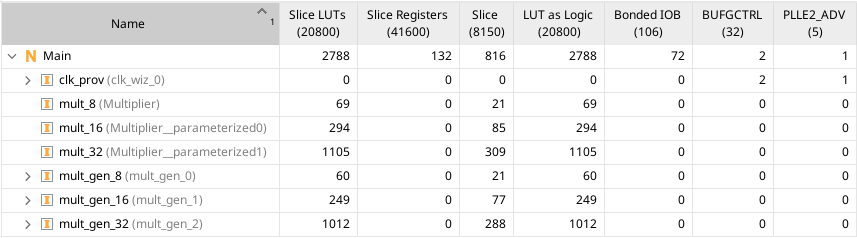
\includegraphics[width=1\linewidth]{images/LUT_MUL_Util.png}
    \centering
    \caption{Only LUT Multilier Utilization Hierarchical}
    \label{fig:only_lut_util}
\end{figure}

The submodules that has 'gen' in their names are IP multipliers build with only LUTs. The results indicate that the IP has better resource utilization than the '*' operator.

\textbf{Power:}
\begin{figure}[ht]
    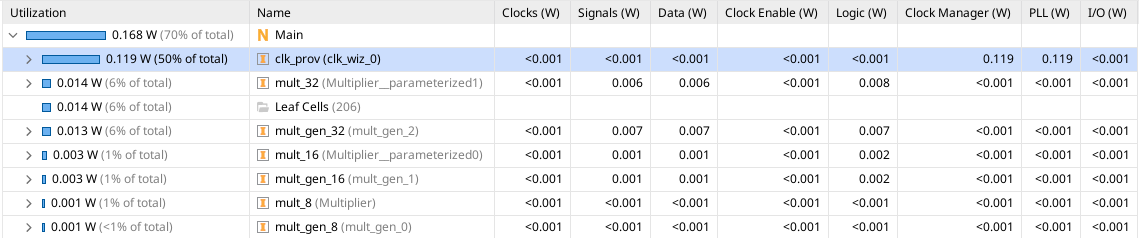
\includegraphics[width=1\linewidth]{images/LUT_MUL_POWER.png}
    \centering
    \caption{Only LUT Multilier Power Hierarchical}
    \label{fig:only_lut_power}
\end{figure}

The results indicates that the IP has better power utilization than the '*' operator.

\textbf{Timing:}
Critical path timing (Violating) of the design as follows:

\begin{verbatim}

a_32_reg Register -> LUT 32 IP -> product_ip_64 Register

Slack (VIOLATED) :        -0.973ns  (required time - arrival time)
  Source:                 a_32_reg[8]/C
                            (rising edge-triggered cell FDRE clocked by clk_out1_clk_wiz_0  {rise@0.000ns fall@5.000ns period=10.000ns})
  Destination:            product_ip_64_reg[63]/D
                            (rising edge-triggered cell FDCE clocked by clk_out1_clk_wiz_0  {rise@0.000ns fall@5.000ns period=10.000ns})
  Path Group:             clk_out1_clk_wiz_0
  Path Type:              Setup (Max at Slow Process Corner)
  Requirement:            10.000ns  (clk_out1_clk_wiz_0 rise@10.000ns - clk_out1_clk_wiz_0 rise@0.000ns)
  Data Path Delay:        10.936ns  (logic 6.760ns (61.812%)  route 4.176ns (38.188%))
  Logic Levels:           23  (CARRY4=18 LUT2=4 LUT4=1)
  Clock Path Skew:        -0.031ns (DCD - SCD + CPR)
    Destination Clock Delay (DCD):    -2.062ns = ( 7.938 - 10.000 ) 
    Source Clock Delay      (SCD):    -2.457ns
    Clock Pessimism Removal (CPR):    -0.425ns
  Clock Uncertainty:      0.068ns  ((TSJ^2 + DJ^2)^1/2) / 2 + PE
    Total System Jitter     (TSJ):    0.071ns
    Discrete Jitter          (DJ):    0.116ns
    Phase Error              (PE):    0.000ns

b_32_reg Register -> LUT 32 '*' Logic -> product_64 Register

Slack (VIOLATED) :        -0.776ns  (required time - arrival time)
  Source:                 b_32_reg[4]/C
                            (rising edge-triggered cell FDRE clocked by clk_out1_clk_wiz_0  {rise@0.000ns fall@5.000ns period=10.000ns})
  Destination:            product_64_reg[63]/D
                            (rising edge-triggered cell FDCE clocked by clk_out1_clk_wiz_0  {rise@0.000ns fall@5.000ns period=10.000ns})
  Path Group:             clk_out1_clk_wiz_0
  Path Type:              Setup (Max at Slow Process Corner)
  Requirement:            10.000ns  (clk_out1_clk_wiz_0 rise@10.000ns - clk_out1_clk_wiz_0 rise@0.000ns)
  Data Path Delay:        10.851ns  (logic 5.250ns (48.381%)  route 5.601ns (51.619%))
  Logic Levels:           21  (CARRY4=15 LUT3=2 LUT4=1 LUT5=1 LUT6=2)
  Clock Path Skew:        0.034ns (DCD - SCD + CPR)
    Destination Clock Delay (DCD):    -2.002ns = ( 7.998 - 10.000 ) 
    Source Clock Delay      (SCD):    -2.462ns
    Clock Pessimism Removal (CPR):    -0.425ns
  Clock Uncertainty:      0.068ns  ((TSJ^2 + DJ^2)^1/2) / 2 + PE
    Total System Jitter     (TSJ):    0.071ns
    Discrete Jitter          (DJ):    0.116ns
    Phase Error              (PE):    0.000ns

a_32_reg Register -> LUT 16 '*' Logic -> product_32 Register
Slack (VIOLATED) :        -0.131ns  (required time - arrival time)
  Source:                 a_32_reg[12]/C
                            (rising edge-triggered cell FDRE clocked by clk_out1_clk_wiz_0  {rise@0.000ns fall@5.000ns period=10.000ns})
  Destination:            product_32_reg[31]/D
                            (rising edge-triggered cell FDCE clocked by clk_out1_clk_wiz_0  {rise@0.000ns fall@5.000ns period=10.000ns})
  Path Group:             clk_out1_clk_wiz_0
  Path Type:              Setup (Max at Slow Process Corner)
  Requirement:            10.000ns  (clk_out1_clk_wiz_0 rise@10.000ns - clk_out1_clk_wiz_0 rise@0.000ns)
  Data Path Delay:        10.134ns  (logic 3.673ns (36.244%)  route 6.461ns (63.756%))
  Logic Levels:           12  (CARRY4=7 LUT3=1 LUT4=1 LUT5=1 LUT6=2)
  Clock Path Skew:        -0.038ns (DCD - SCD + CPR)
    Destination Clock Delay (DCD):    -2.067ns = ( 7.933 - 10.000 ) 
    Source Clock Delay      (SCD):    -2.455ns
    Clock Pessimism Removal (CPR):    -0.425ns
  Clock Uncertainty:      0.068ns  ((TSJ^2 + DJ^2)^1/2) / 2 + PE
    Total System Jitter     (TSJ):    0.071ns
    Discrete Jitter          (DJ):    0.116ns
    Phase Error              (PE):    0.000ns

a_32_reg Register -> LUT 32 '*' IP -> product_ip_32 Register
Slack (VIOLATED) :        -0.104ns  (required time - arrival time)
  Source:                 a_32_reg[0]/C
                            (rising edge-triggered cell FDRE clocked by clk_out1_clk_wiz_0  {rise@0.000ns fall@5.000ns period=10.000ns})
  Destination:            product_ip_32_reg[31]/D
                            (rising edge-triggered cell FDCE clocked by clk_out1_clk_wiz_0  {rise@0.000ns fall@5.000ns period=10.000ns})
  Path Group:             clk_out1_clk_wiz_0
  Path Type:              Setup (Max at Slow Process Corner)
  Requirement:            10.000ns  (clk_out1_clk_wiz_0 rise@10.000ns - clk_out1_clk_wiz_0 rise@0.000ns)
  Data Path Delay:        10.107ns  (logic 5.046ns (49.927%)  route 5.061ns (50.073%))
  Logic Levels:           14  (CARRY4=10 LUT2=4)
  Clock Path Skew:        -0.038ns (DCD - SCD + CPR)
    Destination Clock Delay (DCD):    -2.070ns = ( 7.930 - 10.000 ) 
    Source Clock Delay      (SCD):    -2.458ns
    Clock Pessimism Removal (CPR):    -0.425ns
  Clock Uncertainty:      0.068ns  ((TSJ^2 + DJ^2)^1/2) / 2 + PE
    Total System Jitter     (TSJ):    0.071ns
    Discrete Jitter          (DJ):    0.116ns
    Phase Error              (PE):    0.000ns

\end{verbatim}

The results indicate that 32-bit multiplication has timing violation for both. The '*' operator seems to more close to 0 slack than the IP multiplier for 32-Bit.
However, for the 16-bit violation, the IP multiplier has better slack than the '*' operator. Using LUT multipliers ('*' or IP) over 8-bit is not recommended because of inefficient resource utilization and timing violations.

\subsection{Second Case}
In this case, we will use the '*' operator and Multilier IP (No Stages) to multiply two numbers, using DSPs.

The modules used are below:
\begin{verbatim}
(* USE_DSP="yes", keep_hierarchy = "yes" *) module Multiplier_Dsp #(parameter A_WIDTH = 8,
     B_WIDTH = 8)(input wire clk,
    input wire [A_WIDTH-1:0] a,
    input wire [B_WIDTH-1:0] b,
    output reg [A_WIDTH+B_WIDTH-1:0] product
);

    always @(clk) begin
        product <= a * b;
    end
endmodule
module Main_Dsp(
input wire clk, input wire [31:0] raw_a_32, input wire [31:0] raw_b_32, input wire rst, output reg [5:0] fake_out
    );

    wire AHundredMHz_clk;
    wire TwoHundredMHz_clk;
    wire locked;

    reg [31:0] a_32;
    reg [31:0] b_32;
    reg [15:0] product_16;
    reg [31:0] product_32;
    reg [63:0] product_64;
    reg [15:0] product_ip_16;
    reg [31:0] product_ip_32;
    reg [63:0] product_ip_64;

    clk_wiz_0 clk_prov_1(.clk_out1(AHundredMHz_clk), .clk_out2(TwoHundredMHz_clk), .reset(rst), .locked(locked), .clk_in1(clk));

    wire [15:0] product_w_16;
    wire [31:0] product_w_32;
    wire [63:0] product_w_64;    
    wire [15:0] product_ip_w_16;
    wire [31:0] product_ip_w_32;
    wire [63:0] product_ip_w_64;    

    Multiplier_Dsp #(.A_WIDTH(8), .B_WIDTH(8)) mult_dsp_8(.clk(AHundredMHz_clk), .a(a_32[7:0]), .b(b_32[7:0]), .product(product_w_16));
    Multiplier_Dsp #(.A_WIDTH(16), .B_WIDTH(16)) mult_dsp_16(.clk(AHundredMHz_clk), .a(a_32[15:0]), .b(b_32[15:0]), .product(product_w_32));
    Multiplier_Dsp #(.A_WIDTH(32), .B_WIDTH(32)) mult_dsp_32(.clk(AHundredMHz_clk), .a(a_32[31:0]), .b(b_32[31:0]), .product(product_w_64));

    mult_gen_3 mult_gen_dsp_8(a_32[7:0], b_32[7:0], product_ip_w_16);
    mult_gen_4 mult_gen_dsp_16(a_32[15:0], b_32[15:0], product_ip_w_32);
    mult_gen_5 mult_gen_dsp_32(a_32[31:0], b_32[31:0], product_ip_w_64);

    always @(posedge AHundredMHz_clk or posedge rst) begin
        if (rst) begin
            product_16 <= 16'b0;
            product_32 <= 32'b0;
            product_64 <= 64'b0;
            product_ip_16 <= 16'b0;
            product_ip_32 <= 32'b0;
            product_ip_64 <= 64'b0;
        end
        else begin
            product_16 <= product_w_16;
            product_32 <= product_w_32;
            product_64 <= product_w_64;
            product_ip_16 <= product_ip_w_16;
            product_ip_32 <= product_ip_w_32;
            product_ip_64 <= product_ip_w_64;
            fake_out[0] <= product_16[15];
            fake_out[1] <= product_32[31];
            fake_out[2] <= product_64[63];
            fake_out[3] <= product_ip_16[15];
            fake_out[4] <= product_ip_32[31];
            fake_out[5] <= product_ip_64[63];
            a_32 <= raw_a_32;
            b_32 <= raw_b_32;
        end
    end
endmodule
\end{verbatim}

The results of the second case are shown below:
\textbf{Utilization:}
\begin{figure}[ht]
    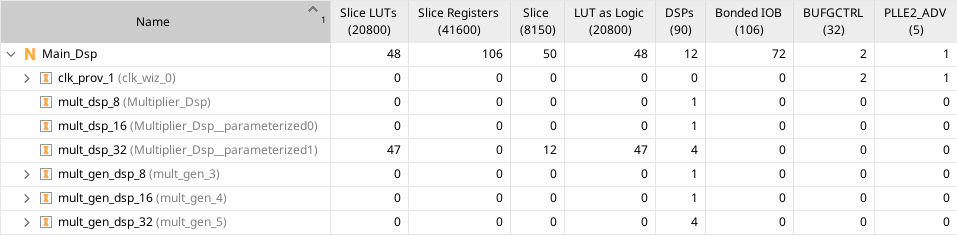
\includegraphics[width=1\linewidth]{images/MUL_DSP_Util.png}
    \centering
    \caption{DSP Multilier Utilization Hierarchical}
    \label{fig:dsp_util}
\end{figure}

The submodules that has 'gen' in their names are IP multipliers built with only DSPs. The results indicate that the IP has better resource utilization than the '*' operator for only 32-bit multiplication. Otherwise same.

\break
\textbf{Power:}

\begin{figure}[ht]
    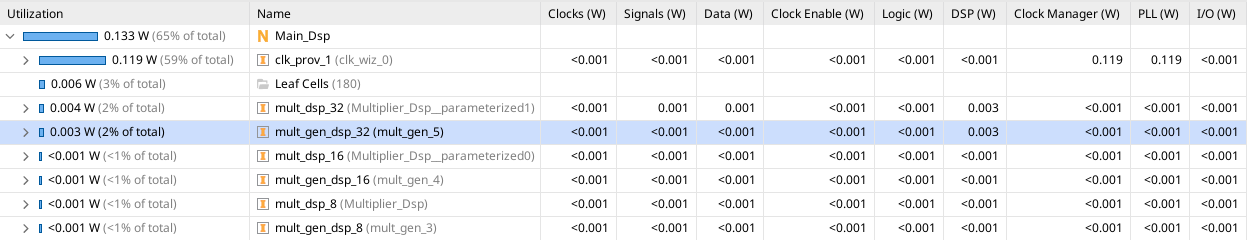
\includegraphics[width=1\linewidth]{images/MUL_DSP_POWER.png}
    \centering
    \caption{DSP Multilier Power Hierarchical}
    \label{fig:dsp_power}
\end{figure}
For 32-bit, IP multiplier has better power utilization than the '*' operator. Otherwise, they are similar.

\textbf{Timing:}
Critical path timing (Violating) of the design as follows:

\begin{verbatim}
Slack (VIOLATED) :        -0.644ns  (required time - arrival time)
  Source:                 a_32_reg[10]_replica/C
                            (rising edge-triggered cell FDRE clocked by clk_out1_clk_wiz_0  {rise@0.000ns fall@5.000ns period=10.000ns})
  Destination:            product_ip_64_reg[63]/D
                            (rising edge-triggered cell FDCE clocked by clk_out1_clk_wiz_0  {rise@0.000ns fall@5.000ns period=10.000ns})
  Path Group:             clk_out1_clk_wiz_0
  Path Type:              Setup (Max at Slow Process Corner)
  Requirement:            10.000ns  (clk_out1_clk_wiz_0 rise@10.000ns - clk_out1_clk_wiz_0 rise@0.000ns)
  Data Path Delay:        10.540ns  (logic 9.436ns (89.525%)  route 1.104ns (10.475%))
  Logic Levels:           4  (DSP48E1=4)
  Clock Path Skew:        -0.020ns (DCD - SCD + CPR)
    Destination Clock Delay (DCD):    -2.061ns = ( 7.939 - 10.000 ) 
    Source Clock Delay      (SCD):    -2.454ns
    Clock Pessimism Removal (CPR):    -0.412ns
  Clock Uncertainty:      0.068ns  ((TSJ^2 + DJ^2)^1/2) / 2 + PE
    Total System Jitter     (TSJ):    0.071ns
    Discrete Jitter          (DJ):    0.116ns
    Phase Error              (PE):    0.000ns

    
Slack (VIOLATED) :        -0.068ns  (required time - arrival time)
  Source:                 b_32_reg[6]_replica/C
                            (rising edge-triggered cell FDRE clocked by clk_out1_clk_wiz_0  {rise@0.000ns fall@5.000ns period=10.000ns})
  Destination:            product_64_reg[63]/D
                            (rising edge-triggered cell FDCE clocked by clk_out1_clk_wiz_0  {rise@0.000ns fall@5.000ns period=10.000ns})
  Path Group:             clk_out1_clk_wiz_0
  Path Type:              Setup (Max at Slow Process Corner)
  Requirement:            10.000ns  (clk_out1_clk_wiz_0 rise@10.000ns - clk_out1_clk_wiz_0 rise@0.000ns)
  Data Path Delay:        10.043ns  (logic 7.611ns (75.785%)  route 2.432ns (24.215%))
  Logic Levels:           10  (CARRY4=7 DSP48E1=2 LUT2=1)
  Clock Path Skew:        -0.019ns (DCD - SCD + CPR)
    Destination Clock Delay (DCD):    -2.061ns = ( 7.939 - 10.000 ) 
    Source Clock Delay      (SCD):    -2.455ns
    Clock Pessimism Removal (CPR):    -0.412ns
  Clock Uncertainty:      0.068ns  ((TSJ^2 + DJ^2)^1/2) / 2 + PE
    Total System Jitter     (TSJ):    0.071ns
    Discrete Jitter          (DJ):    0.116ns
    Phase Error              (PE):    0.000ns
\end{verbatim}

The results indicate that 32-bit multiplication has timing violation for both. The '*' operator seems to more close to 0 slack than the IP multiplier for 32-Bit.
When other met max delay paths are inspected, the IP multiplier data path delay is larger than '*' in general.
For a no stage multiplication using DSP a '*' operator might be the choice for better slack given a bit more area is used.

Given the results using DSP blocks are much more efficient than using LUTs for multiplication for larger bit arrays.
If the design intends to use no pipeline, the '*' operator might be the choice for better slack and usage simplicity as the results are close with no stage IP. 

\section{Slack / Clock / Pipeline Relationship Investigation}
In this part we will try to answer following questions: 
\begin{enumerate}
    \item Can we assume that if we increase clock period by X seconds, slack will increase by X seconds?
    \item How does Multiplier IP stages effect slack? (Even delay paths between stages or not)
    \item Using the information from first two questions, can we fine tune the clock period given to IP multiplier to have a single clock cycle result in the top module?
    \item Why does the IP setup suggests a stage level? Is it related to the maximum clock speed of the device?
\end{enumerate}

\subsection{First Question}
In this part, we will try to understand the relationship between slack and clock period. We will try to increase the clock period by X seconds and see if the slack increases by X seconds.
We will use the same module from the dsp part of the multiplication part using only IP Multiliers.

The clock period was set to 10ns and worst slack was around -0.644ns. New clock period will be:
\[
\text{Closest integer} = \left\lfloor \frac{1}{10 \, \text{ns} + 0.644} + \frac{1}{2} \right\rfloor = 93896714 \approx 93.75 \text{MHZ}
\]
The hypothesis is that if we set the clock period to 10.667ns, the slack will be positive close to 0. The results are shown below:
\begin{verbatim}
    -------------------------------------------------------------------
    required time                          8.073    
    arrival time                          -8.073    
-------------------------------------------------------------------
    slack                                 -0.001
\end{verbatim}
It failed again. It is observed that the slack is close to 0. The hypothesis is close to be correct. The slack is increased by 0.649ns when the clock period is increased by 0.667ns. Given the phase error and jitter of the clock it is more safe to increase the clock period more than required.

Trying again with 93.333MHZ, 10.71ns:

\begin{verbatim}
    -------------------------------------------------------------------
    required time                          8.117    
    arrival time                          -8.076    
-------------------------------------------------------------------
    slack                                  0.041    
\end{verbatim}
Slack is tested again with other clocks as data path delay is changing with the clock When the results are combined (Note that the non ip parts are removed therefore the the slack at 100MHZ is different than the previous results):

\text{}

\begin{table}[!h]
    \centering
    \caption{Timing Analysis at Different Clock Frequencies}
    \begin{tabular}{|c|c|c|c|}
    \hline
    \textbf{Path Delay} & \textbf{Clk frq (MHz)} & \textbf{Period (ns)} & \textbf{Slack} \\
    \hline
    11.093 & 50       & 20.000   & 8.657     \\
    10.538 & 93.333   & 10.714   & 0.041     \\
    10.535 & 93.750   & 10.535   & -0.001    \\
    10.373 & 100      & 10.000   & -0.495    \\
    10.361 & 200      & 5.000    & -5.488    \\
    \hline
    \end{tabular}
    \end{table}

By looking and plotting the data we can see that the data path delay and thus the slack values are not linearly related to the clock period.
As frequency increases, the path delay change descreases.
By doing this analysis we can conclude that there is no linear relationship between slack and clock period, but there is a relation this close to linear at higher clock speeds.

\subsection{Second Question}
The second question requires us to find how does Multiplier IP pipelines multiple stages.
To find a relationship, we will use critical path and how it is reduced after each stage. Same module will be used with different stages of IP multipliers.

During this test we will use 10ns clock period. It has initially Worst Slack as -0.495ns.
The two paths that are critical are:
\begin{itemize}
    \item any a or b register to IP (it can have a weird name like mult\_gen\_dsp\_32/U0/i\_mult/gDSP.gDSP\_only.iDSP/ use\_prim.appDSP[1].bppDSP[1].use\_dsp.use\_dsp48e1.iDSP48E1/PCIN[0]) which refers to a flip flop inside the DSP block)
    \item any path from IP to output register 
    \item any path from IP register to IP register
\end{itemize}

\begin{enumerate}
    \item \textbf{Stage 0:} Slowest path is from a\_32[i] register to the product register through the IP. \textbf{The max data path delay is 10.373 ns.}
    \item \textbf{Stage 1:} Slowest path is from a\_32[i] register to a dsp register register inside the IP. \textbf{Data path delay is 8.503.} Searching a path from an IP to output register, \textbf{the longest path is 1.119ns} and it is in the 32-bit multiplier. It suggests that the IP doing most of the job in the first cycle.
    \item \textbf{Stage 2:} Slowest path is from a dsp register inside the IP to a dsp register register inside the IP (mult\_gen\_dsp\_32/U0/i\_mult/gDSP.gDSP\_only.iDSP/use\_prim.appDSP[0].bppDSP[0].use\_dsp.use\_dsp48e1.iDSP48E1/CLK to mult\_gen\_dsp\_32/U0/i\_mult/gDSP.gDSP\_only.iDSP/use\_prim.appDSP[1].bppDSP[1]). \textbf{Data path delay is 6.633.}. It suggests that most of the job is done in the intermediate cycle. In the first cycle the maximum data path is to the 32-bit multiplier IP and \textbf{Its data path delay is 2.815.} The maximum data path delay from the IPs to output register is 1.180ns and in the 32-bit multiplier.
    \item \textbf{Stage 3:} From timing report couldn't detect pipelining paths due to hidden information, but intermediate maximum data path delay is \textbf{4.208ns}. Input to the IP paths has maximum delay \textbf{2.815 ns}. The maximum data path delay from the IPs to output register is \textbf{1.119ns.} These are the maximum delay paths and they are inside the 32-bit multiplier IP.
\end{enumerate}

From this infromation we can come up with a table:

\begin{table}[h!]
    \centering
    \begin{tabular}{c|c|c|c}
    \toprule
    & \multicolumn{3}{c}{Critical Path Delays (ns)} \\
    \midrule
    \# of Stages  & Input & Intermediate Step/s & Output \\
    \midrule
    0 & \multicolumn{3}{c}{Combinational* \hspace{30pt} 10.373} \\
    \midrule
    1 & 8.503 & - & 1.119 \\
    \midrule
    2 & 2.815 & 6.633 & 1.180 \\
    \midrule
    3 & 2.815 & 4.208 & 1.119 \\
    \bottomrule
    \end{tabular}
    \caption{Critical Path Delays}
    \label{tab:critical_path_delays}
    \end{table}
Input refers to the delay from the input register to the IP, intermediate step/s refers to the delay inside the IPs, and output refers to the delay from the IP to the output register.
A few things can be inferred from the table:
\begin{itemize}
    \item The maximum delay path is reduced after each stage by around 2ns.
    \item Stages are not divided equally. An intermediate step is doing most of the job, or first one if it is a stage 0 and stage 1 IP.
    \item After 2 stages data path that gets input and gives output stays similar as job is done in the intermediate steps. 
\end{itemize}

To be sure that the data path delay is reduced by 2ns after each stage, the reports for 4 stages and check the data path delays is checked. The maximum delay path in the ip and the whole system reduced to 2.428 as expected. At 5th stage, intermediate step path delays are below input and output path delays and \textbf{almost all of their delays are net delay}, so we can't say at every stage 2ns reduced.

\subsection{Third Question}
The investigation indicates that we can't assume that the stages are equally divided and we cannot multiply clock by 2 as we increase the pipeline stages by one.
\subsection{Fourth Question}
Another mistery that why and how the optimum stage level of multiplier ip suggested by Vivado. The hypothesis is that it is related to the minimum clock period that the device, Basys3, can handle. Basys3 can handle maximum \textbf{450MHZ} clock frequency as documented, which corresponds to 2.222ns. The IP suggests a stage level to be 6 for 32-bit unsigned multiplier. We will check:
\begin{itemize}
    \item The maximum delay path and the slack in the IP at stage level suggested.
    \item If it is below 2.222ns and we have slack around 8ns, we will check slack given the clock period is 2.222ns because given clock related time delays data path delay doesn't directly mean time required.
    \item To finalize the hypothesis, we will check again at stage level 5 if it is failing timing.
\end{itemize}

\textbf{Checking at Stage Level 6:}
The result showted that the worst data path delay in the whole system is 2.585ns. Minimum slack is 6.852. However, higher clock speeds can make the dsp even faster as we already found. Therefore it is worth to check the slack at 2.222ns clock period.

\textbf{Checking at 2.222ns Clock Period:}
The results indicate that the design got faster. The worst path delay is 1.802. However, due to clock effects it is slightly negative, -0.045ns. Which means that we can try to work with 400MHZ clock.

\textbf{Checking at 2.5ns Clock Period:}
After decreasing frequency to 400MHZ, worst slack is:
\begin{verbatim}
        Slack (MET) :             0.014ns  (required time - arrival time)
        -------------------------------------------------------------------
                         required time                         -0.667    
                         arrival time                           0.681    
  -------------------------------------------------------------------
                         slack                                  0.014    
\end{verbatim}

This test indicted that the optimum suggested stage level is related to the maximum clock speed of the device. The IP suggests a stage level that can handle the maximum clock speed of the device. Due to clock uncertainty it is same to use a smaller clock period than the maximum clock speed of the device as slack report showed. The report showed clock uncertainty and adds it to time domain to find the slack:
\begin{verbatim}
    Clock Uncertainty:      0.057ns  ((TSJ^2 + DJ^2)^1/2) / 2 + PE
    Total System Jitter     (TSJ):    0.071ns
    Discrete Jitter          (DJ):    0.090ns
    Phase Error              (PE):    0.000ns
\end{verbatim}
This is why at 450MHZ clock period, the slack was negative. The clock uncertainty is 0.057ns and the slack was -0.045ns.



\end{document}



